% !TEX TS-program = xelatex
%
\documentclass[aspectratio=1610]{beamer}

\usetheme{metropolis}

\usepackage{fontspec}
\defaultfontfeatures{Ligatures=TeX}

\usefonttheme{professionalfonts}
\usepackage[familydefault,light]{Chivo}

\usepackage{graphicx}
\usepackage{graphbox}
\graphicspath{ {../assets/} }

\hypersetup
{
  pdftitle  = {IoT Data Analytics using Serverless Computing},
  pdfauthor = {Michael Kaltschmid \& Markus Reiter}
}

\title{IoT Data Analytics using Serverless Computing}
\author{Michael Kaltschmid \& Markus Reiter}
\date{}

\begin{document}
  \maketitle

  \begin{frame}{Outline}
    \begin{itemize}
      \item Introduction
      \item Devices
      \item Serverless Stack
      \item Mobile Application
      \item Web Application
      \item Schedule
    \end{itemize}
  \end{frame}

  \begin{frame}{Introduction}
    \begin{itemize}
      \item collect IoT data from various devices
      \item devices post data to broker
      \item serverless function called depending on data type
      \item data saved in database
      \item web application to visualize data and statistics
    \end{itemize}
  \end{frame}

  \begin{frame}{Devices: Smartphone}
    \begin{itemize}
      \item gyroscope
            \hspace*{2em}
            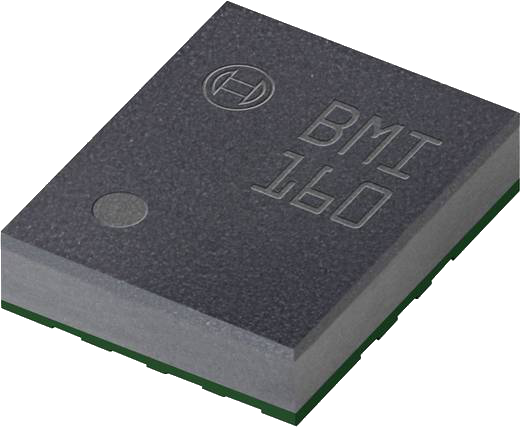
\includegraphics[align=c,height=3em]{bmi160-sensor}
      \item accelerometer
      \item magnetometer
      \item barometer
            \hspace*{2em}
            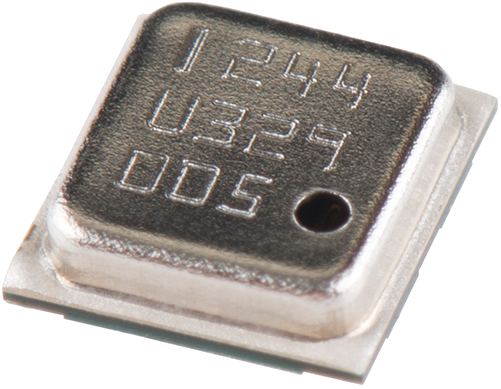
\includegraphics[align=c,height=3em]{barometric-sensor}
      \item gravity
      \item temperature
      \item humidity
            \hspace*{2em}
            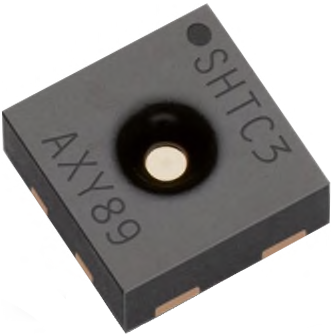
\includegraphics[align=c,height=3em]{shtc3-humidity-sensor}
      \item possibly GPS location
    \end{itemize}
  \end{frame}

  \begin{frame}{Devices: Raspberry Pi}
    \begin{itemize}
      \item temperature sensor
            \hspace*{2em}
            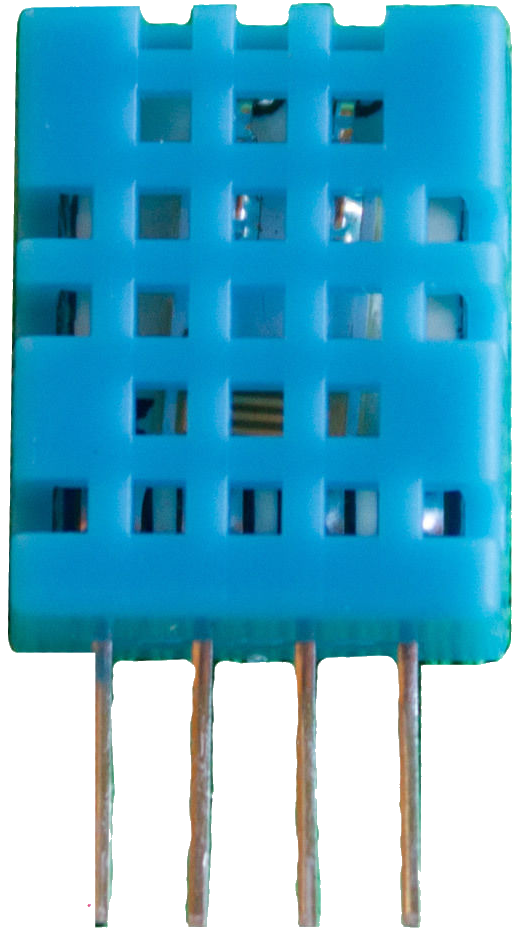
\includegraphics[align=c,height=5em]{dht11-sensor}
      \item humidity sensor
      \item magnetic hall sensor
            \hspace*{2em}
            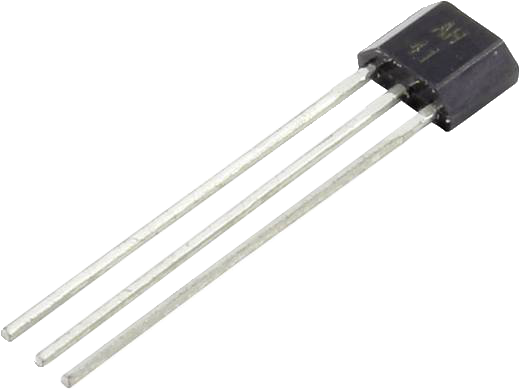
\includegraphics[align=c,height=4em]{hall-sensor}
      \item light intensity sensor
            \hspace*{2em}
            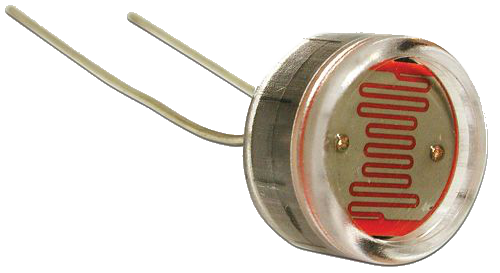
\includegraphics[align=c,height=2em]{light-sensor}
    \end{itemize}
  \end{frame}

  \begin{frame}{Serverless Stack - OpenFaaS}
    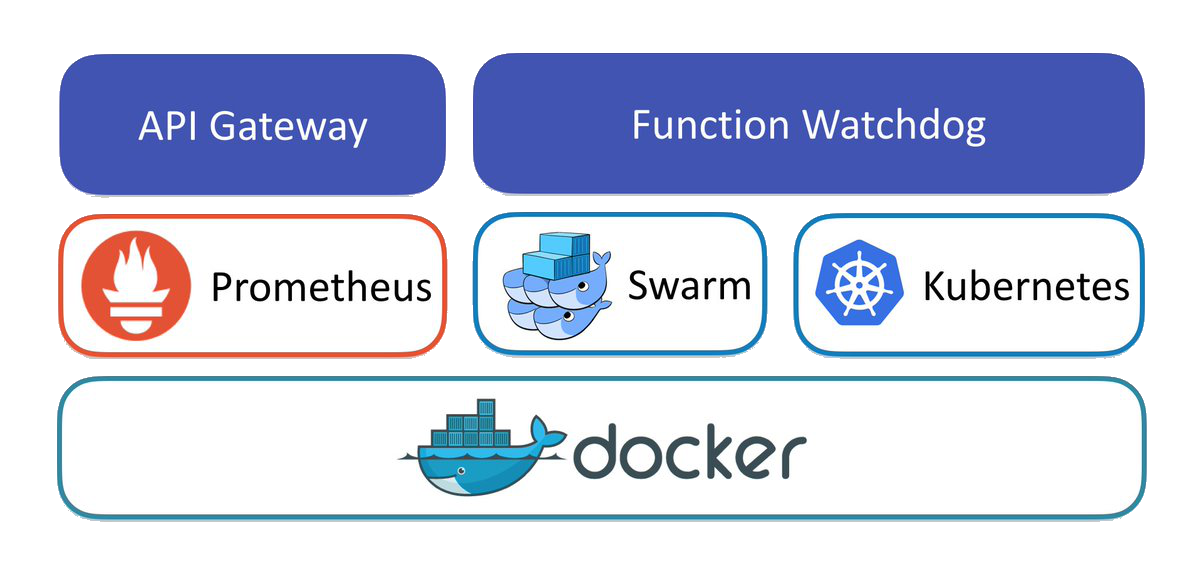
\includegraphics[width=\textwidth]{openfaas-stack}
  \end{frame}

  \begin{frame}{Serverless Stack - Kafka / Zookeeper}
    
\includegraphics[height=6em]{kafka-logo}

    \vspace*{1.5em}

    \begin{itemize}
      \item devices post data to broker
      \item combines data streams
      \item triggers serverless functions
    \end{itemize}
  \end{frame}

  \begin{frame}{Serverless Stack - MongoDB}
    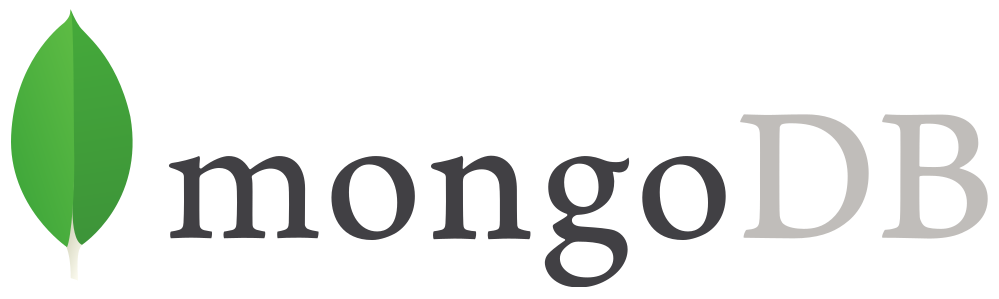
\includegraphics[height=5em]{mongodb-logo}

    \vspace*{1.5em}

    \begin{itemize}
      \item versatile due to its JavaScript origin
      \item persistence layer for sensor data
    \end{itemize}
  \end{frame}

  \begin{frame}{Serverless Stack - Rust}
    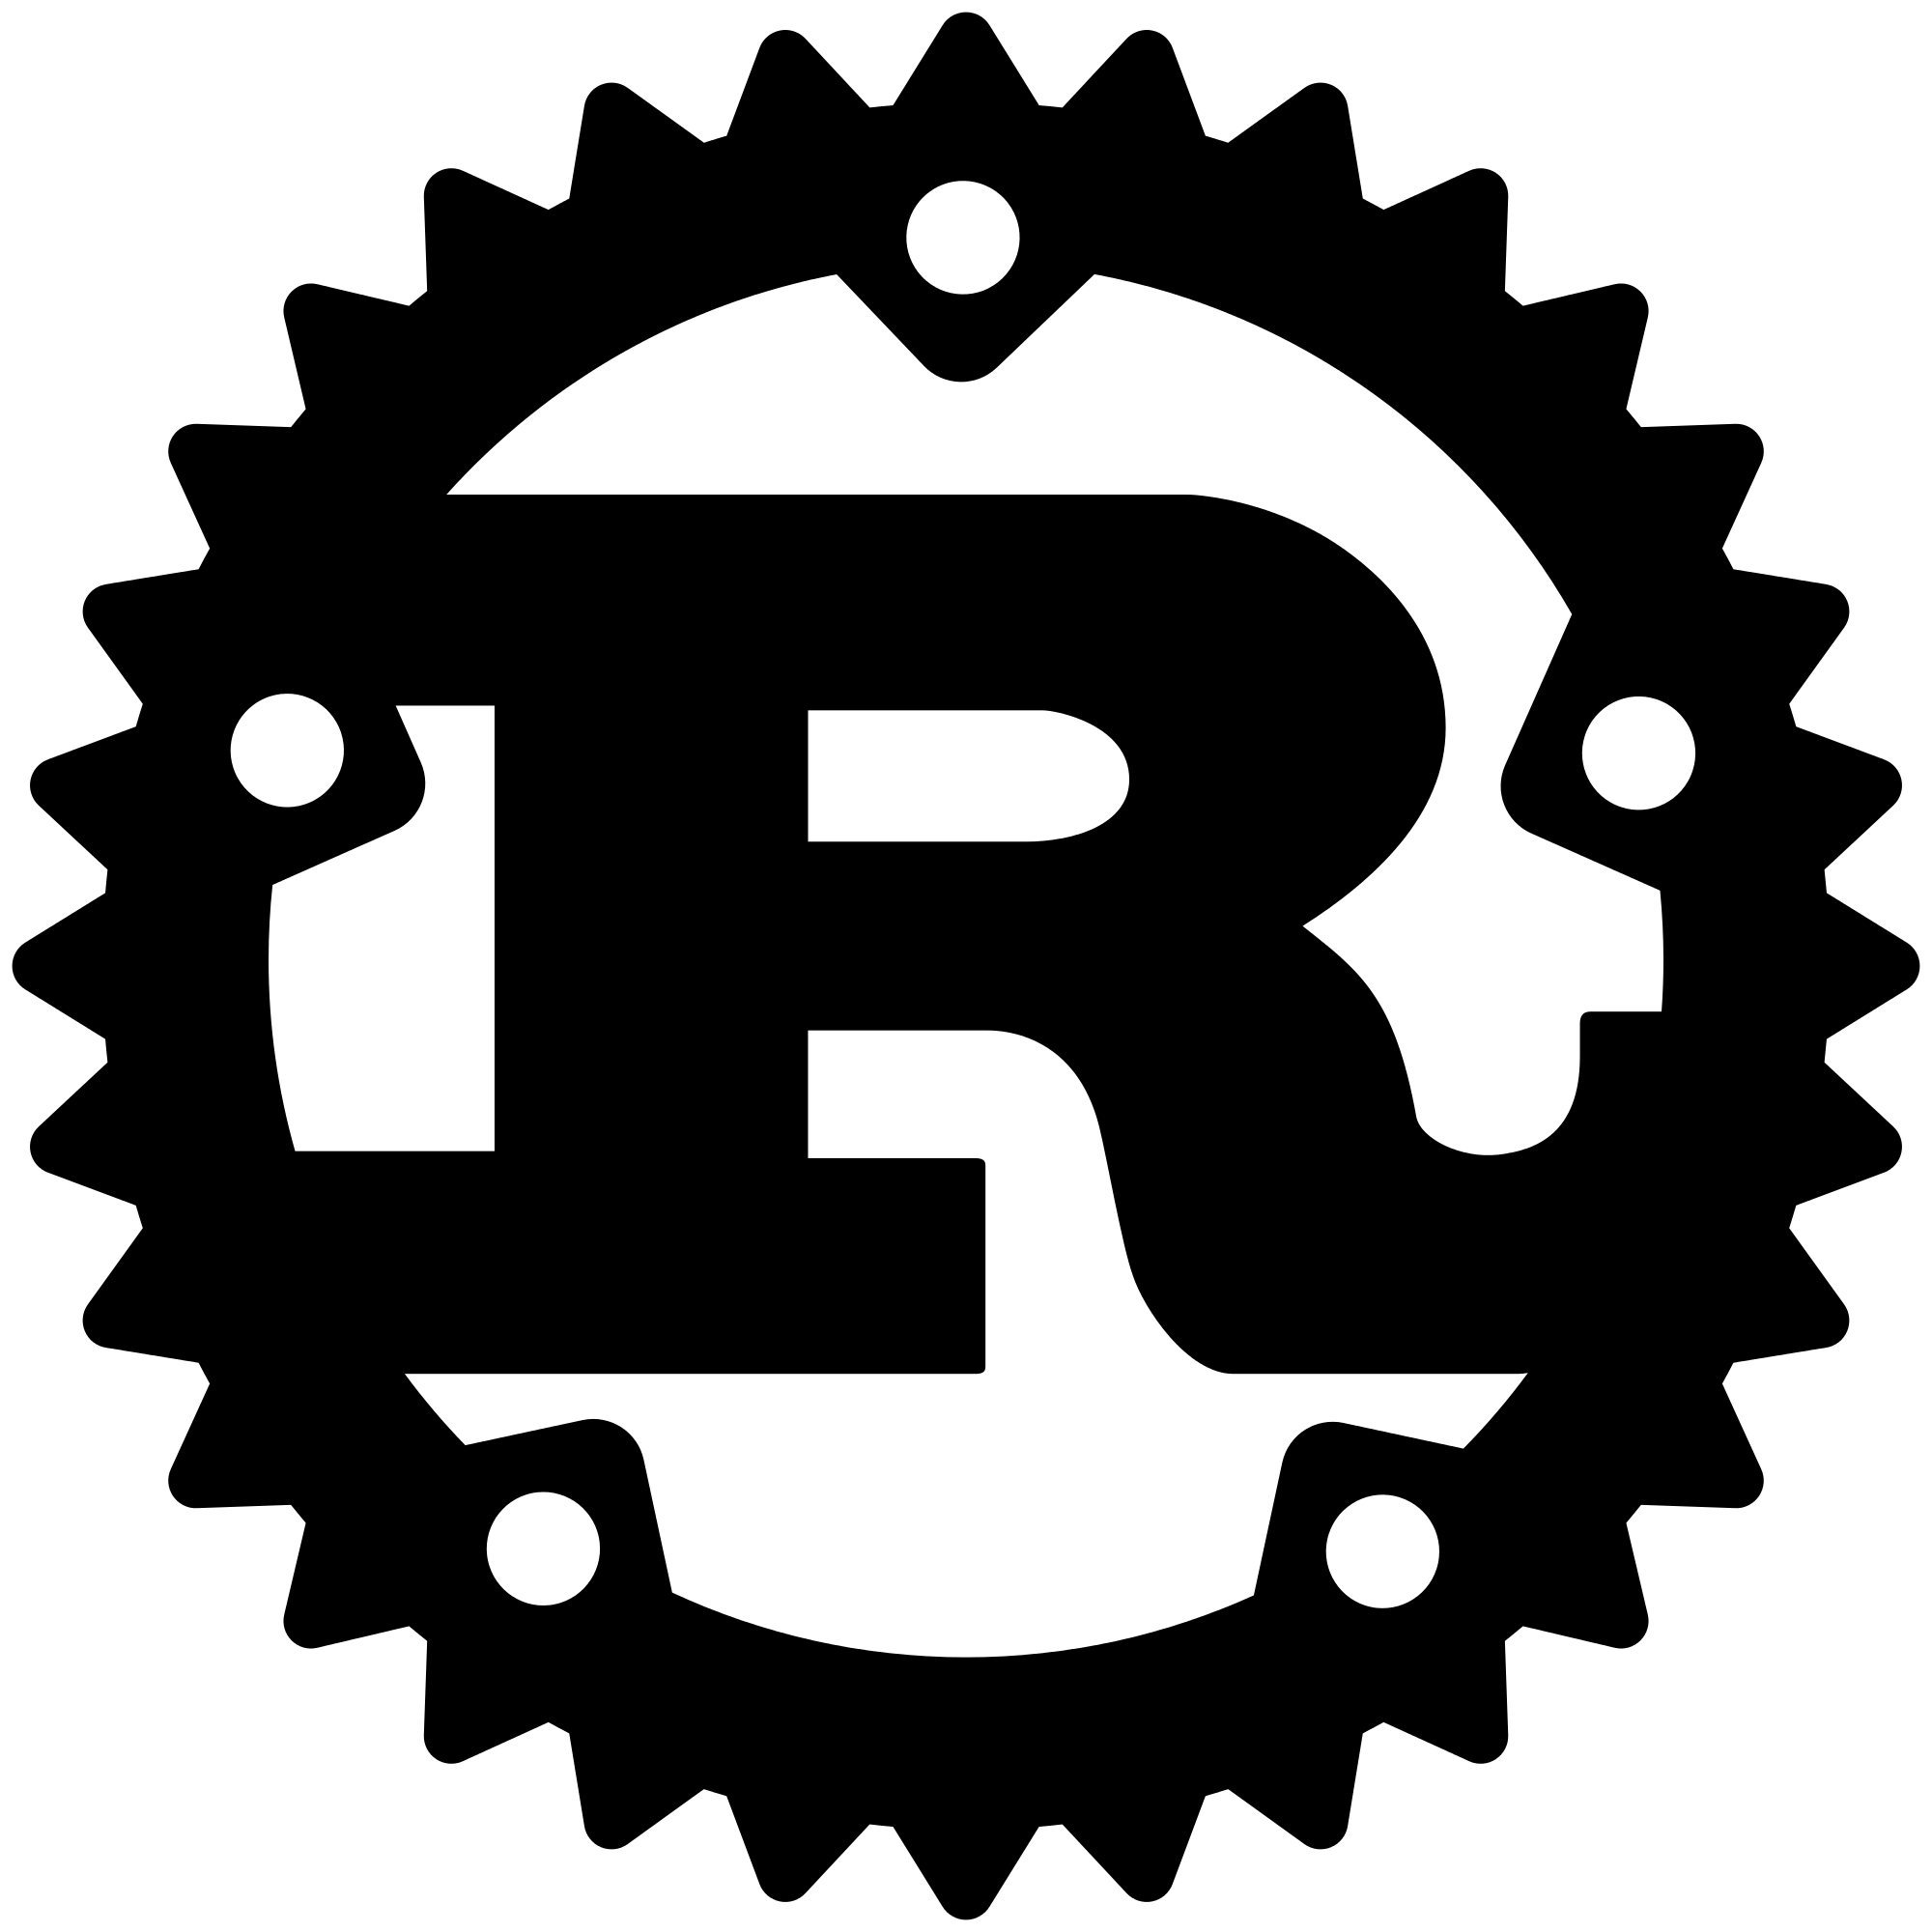
\includegraphics[height=6em]{rust-logo}

    \vspace*{1.5em}

    \begin{itemize}
      \item safe
      \item concurrent
      \item performant
    \end{itemize}
  \end{frame}

  \begin{frame}{Mobile Application}
    
\includegraphics[align=c,height=6em]{android-logo}
    \hspace*{2em}
    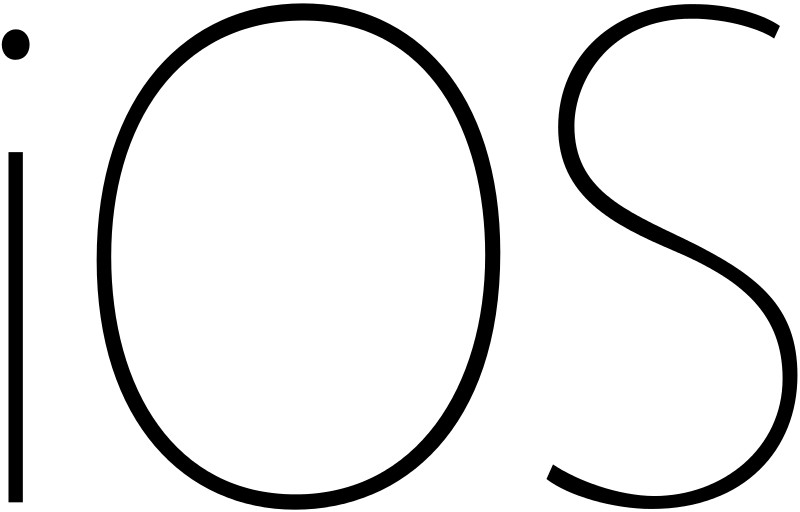
\includegraphics[align=c,height=4em]{ios-logo}

    \vspace*{2em}

    \begin{itemize}
      \item cross plattform using React Native
      \item possible complications on iOS
    \end{itemize}
  \end{frame}

  \begin{frame}{Web Application}
    
\includegraphics[height=6em]{marko-logo}

    \vspace*{2em}

    \begin{itemize}
      \item implemented in Marko
      \item fetching data from MongoDB
      \item reactive interface for all devices
    \end{itemize}
  \end{frame}

  \begin{frame}{Schedule}
    \begin{itemize}
      \item March
        \begin{itemize}
          \item setup serverless stack
          \item start mobile application
        \end{itemize}
      \item April
        \begin{itemize}
          \item finish mobile application
          \item start web application
        \end{itemize}
      \item May
        \begin{itemize}
          \item finish web application
          \item start written part
        \end{itemize}
      \item June
        \begin{itemize}
          \item finalize bachelor’s thesis
        \end{itemize}
    \end{itemize}
  \end{frame}
\end{document}
